\chapter{Experimentelle Ergebnisse}
\label{chap:results}
	In diesem Kapitel wird detailliert geschildert, auf welche Weise die Experimente mit der Differentiellen Evolution durchgeführt worden sind. Im Anschluss werden die daraus erzielten Ergebnisse präsentiert und interpretiert.
	
	\section{Testbedingungen}
	\label{sec:execution}
	
		\subsection{Auswahl an Bildmaterial}
		\label{sub:choice-of-images}
			Zur Evaluierung der Differenziellen Evolution werden insgesamt 30 Bilder herangezogen. Davon weisen 15 Bilder einen laser gravierten Zeichencode wie in Abbildung \ref{fig:example-code}a auf, während die restlichen 15 Bilder einen gestempelten Code nach dem Muster aus \ref{fig:example-code}b vorweisen. Jedes Bild wird dabei zweimal ausgewertet: einmal mit und einmal ohne Mittelwertfilter.\\
			Der Unterschied zwischen den jeweiligen Bildern ist in Abbildung \ref{fig:filter} wiedergegeben:
			\begin{figure}[H]
				\centering
				\subfloat[][Bauteil mit gelasertem Code ohne Mittelwertfilter]{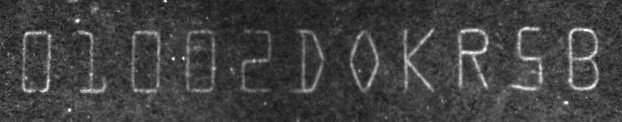
\includegraphics[width=0.48\linewidth]{IMG_01002DOKR5B_c}}
				\quad
				\subfloat[][Bauteil mit gelasertem Code mit Mittelwertfilter]{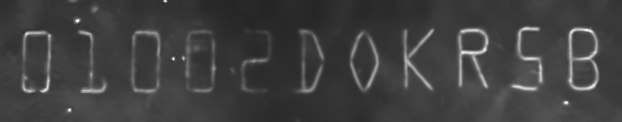
\includegraphics[width=0.48\linewidth]{IMG_01002DOKR5B_c-denoised}}
				
				\subfloat[][Bauteil mit gestempeltem Code ohne Mittelwertfilter]{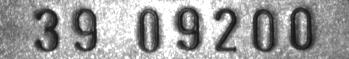
\includegraphics[width=0.48\linewidth]{IMG_3909200}}
				\quad
				\subfloat[][Bauteil mit gestempeltem Code mit Mittelwertfilter]{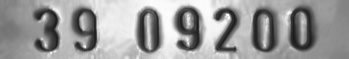
\includegraphics[width=0.48\linewidth]{IMG_3909200-denoised}}
				\caption{Unterschied zwischen Bildern ohne und Bildern mit Mittelwertfilter}
				\label{fig:filter}
			\end{figure}
	
		\subsection{Parameter-Wahl}
		\label{sub:de-params}
			Die einstellbaren Parameter für den implementierten Algorithmus der Differenziellen Evolution und die nachfolgende Segmentierung setzen sich wie folgt zusammen:\\
			Die für den Algorithmus relevanten Parameter belaufen sich auf den Mutationsfaktor $F$, den Crossover-Faktor $C_{r}$ und die maximale Anzahl an Iterationen $G$. Im vorliegenden Test-Szenario wurden $F = 0.5$ und $C_{r} = 0.9$ gewählt. Den Parameter $G$ betreffend wurde eine Unterscheidung getroffen zwischen den Segmentierungsmodellen in den Abschnitten \ref{sub:meth1} und \ref{sub:meth2} respektive. Dementsprechend wurden mit dem Modell der Gaußschen Approximation vier Durchläufe mit $G \in \{100, 200, 500, 1000\}$ ausgeführt, wohingegen anhand des K-Means-Clustering-Modells wegen des deutlich erhöhten Rechenaufwandes im Vergleich mit der Gaußschen Approximation lediglich drei Ausführungssequenzen mit $G \in \{5, 10, 20\}$ absolviert wurden.\\
			In dieser Konstellation werden die Tests für eine Segmentierung in $K$ Klassen mit $K \in \{2,3,4,5\}$ durchgeführt.

	\section{Implementierung der Test-Applikation}
	\label{sec:implementation}
		\subsection{Workflow}
		\label{sub:workflow}
			\begin{figure}[H]
				\centering
				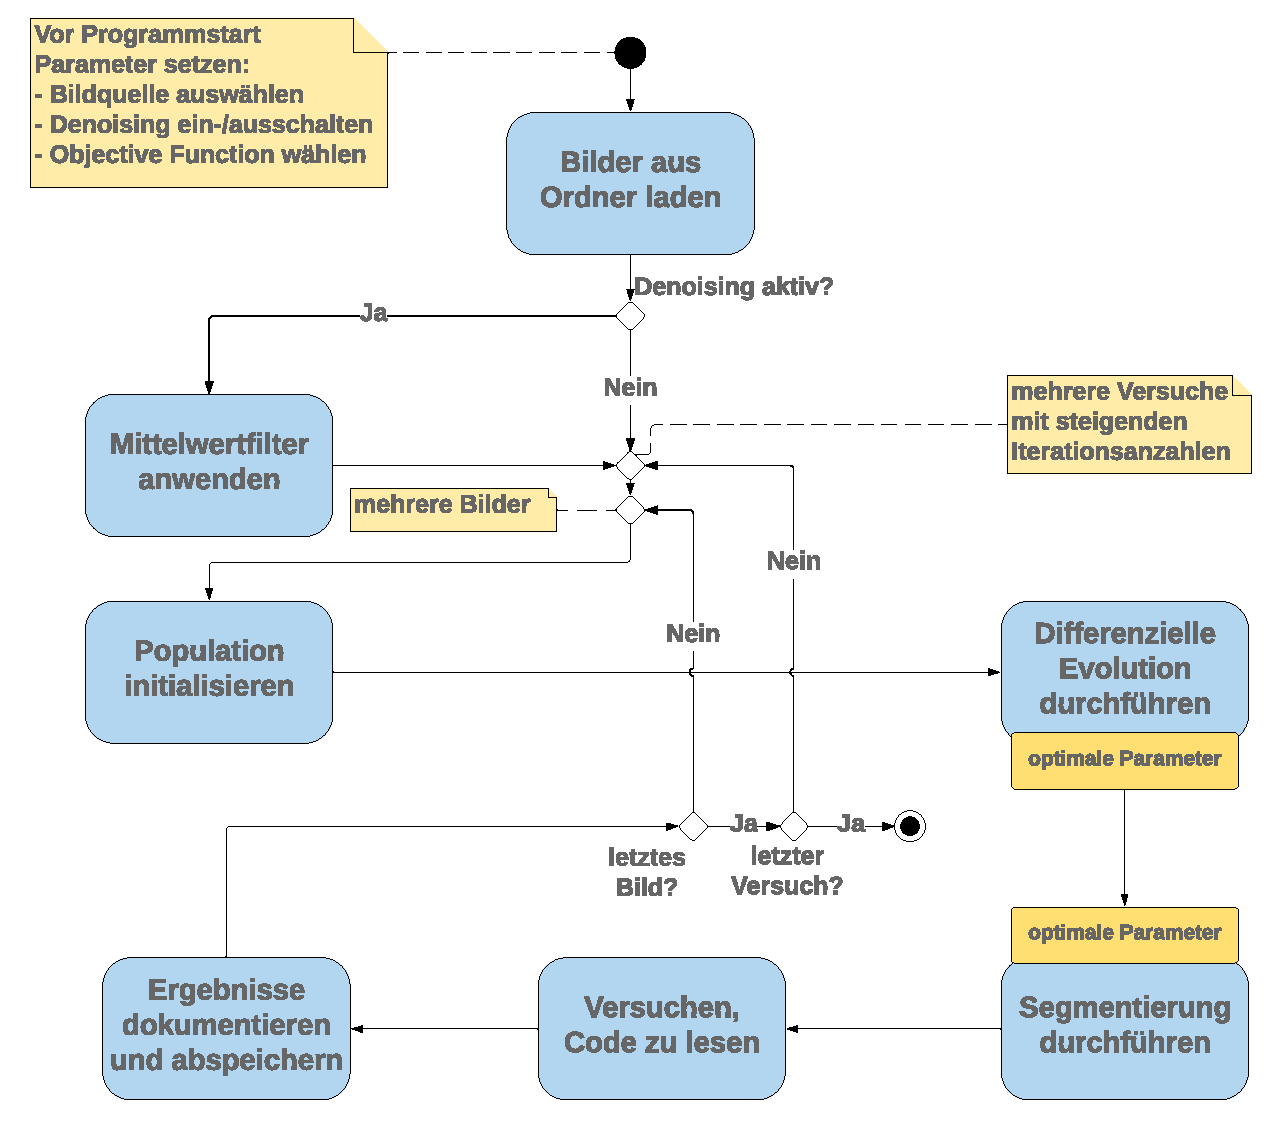
\includegraphics[width=\linewidth]{diff-evol-activity}
				\caption{Aktivitätsdiagramm des Ablaufs in der Test-Applikation}
				\label{fig:diff-evol-activity}
			\end{figure}
			Aus Abbildung \ref{fig:diff-evol-activity} lassen sich die Abläufe entnehmen, die im während dieser Arbeit entwickelten Test-Programm abgehandelt werden:\\
			Vor dem Programmstart muss die Wahl der Bildquelle und des Segmentierungsmodells (künftig als \textit{Objective Function} bezeichnet) getroffen werden. Zusätzlich wird festgelegt, ob ein Mittelwertfilter angewendet werden soll. \\
			Bei Programmstart werden sodann die entsprechenden Bilder geladen und gegebenenfalls mit dem Mittelwertfilter vorbehandelt. Nach diesen Vorbereitungen wird für jedes geladene Bild die Population initialisiert und dem \gls{de}-Algorithmus übergeben. Dieser wird wiederum sukzessiv für jedes $G$, wie in Paragraph \ref{sub:de-params} beschrieben, aufgerufen. Mit dem Ergebnis aus jedem Durchlauf wird dann eine Segmentierung des Bildes anhand der zuvor gewählten \textit{Objective Function} durchgeführt und es folgt ein Versuch, den Code zu lesen. Das jeweilige Resultat hieraus wird schließlich in einer \textit{CSV-Datei} dokumentiert.
	
		\subsection{Wahl der Programmiersprache}
		\label{sub:prog-lang}
			Auf dem Gebiet der Bildverarbeitung haben sich im Allgemeinen zwei Programmiersprachen bewährt - \textit{Python} und \textit{C++} - nicht zuletzt wegen der in der Praxis oft verwendeten Open-Source-Bibliothek \textit{OpenCV}, die für diese beiden Sprachen eine Anwendungsschnittstelle bereitstellt (siehe Online-Dokumentation). Für diese Arbeit ist die Wahl auf die Sprache Python gefallen, da sie gegenüber C++ einige Vorteile mit sich bringt \cite[S. 21f]{python-book}:\\
			Es bietet erhöhte Lesbarkeit sowie Benutzbarkeit aufgrund der Loslösung von der darunterliegenden physischen Schicht. Oft beträgt der Umfang eines Python-Skripts lediglich bis zu einem Drittel der Größe eines äquivalenten C++-Programms. Somit lassen sich mit Python auch komplexere Applikationen in einem kürzeren Zeitrahmen erstellen als mit C++. 

		\subsection{Benutzte Module}
		\label{sub:used-modules}
			Nachstehend ist eine Auflistung jener hier verwendeten Python-Module, die essenziell für die Anfertigung dieser Arbeit waren, zum Zwecke der Nachvollziehbarkeit zu finden:\\
			Für diverse Plots, wie sie in Abschnitt \ref{sec:results} zu finden sind, wurde das \textit{mathplotlib}-Modul \cite[Version 3.1.0]{hunter2007matplotlib} eingesetzt. Für die dieser Arbeit zugrundeliegende Aufgabe war unter anderem das \textit{numpy}-Package \cite[Version 1.16.4]{oliphant2006guide} unabdingbar. Es bietet eine umfangreiche array-ähnliche Datenstruktur, womit sich vor allem Matrix-Operationen mit geringem Aufwand realisieren lassen. So können auch Bilder durch ein zweidimensionales \textit{numpy}-Array dargestellt werden. Zudem sind verschiedene Module mit dem \textit{numpy}-Array kompatibel bzw. sind in der Lage, dieses zu verarbeiten. Hierunter fallen die in der Testapplikation ebenfalls verwendeten Module \textit{scipy} für wissenschaftliche und statistische Kalkulationen \cite[Version 1.2.1]{scipy} sowie das in der Bildverarbeitung präsente \textit{OpenCV} \cite{2014opencv}, das zahlreiche Bildoperationen wie Filter etc. erlaubt. Ebenso sollte \textit{tesserocr} nicht unerwähnt bleiben. Hierbei handelt es sich um einen Python-Wrapper für die Tesseract-\gls{ocr}-Software \cite{tesseract}.
			
	\section{Ergebnisse}
	\label{sec:results}
	
		\subsection{Vergleich Modell 1 - Modell 2}
		\label{sub:comp-m1-m2}
			Die Resultate zeigen hier ein relativ deutliches Ergebnis: allgemein kann darauf geschlossen werden, dass eine Zeichenerkennung mithilfe von Modell 1 mit dem zur Verfügung stehenden Bildmaterial besser funktioniert als mit Modell 2. Ersteres liegt mit einer Erfolgsrate von etwa 18\% knapp mehr als vier mal so hoch wie das zweitere mit lediglich 4\%.
			\begin{figure}[H]
				\centering
				\subfloat[][K=2, G=100, Modell 1 ]{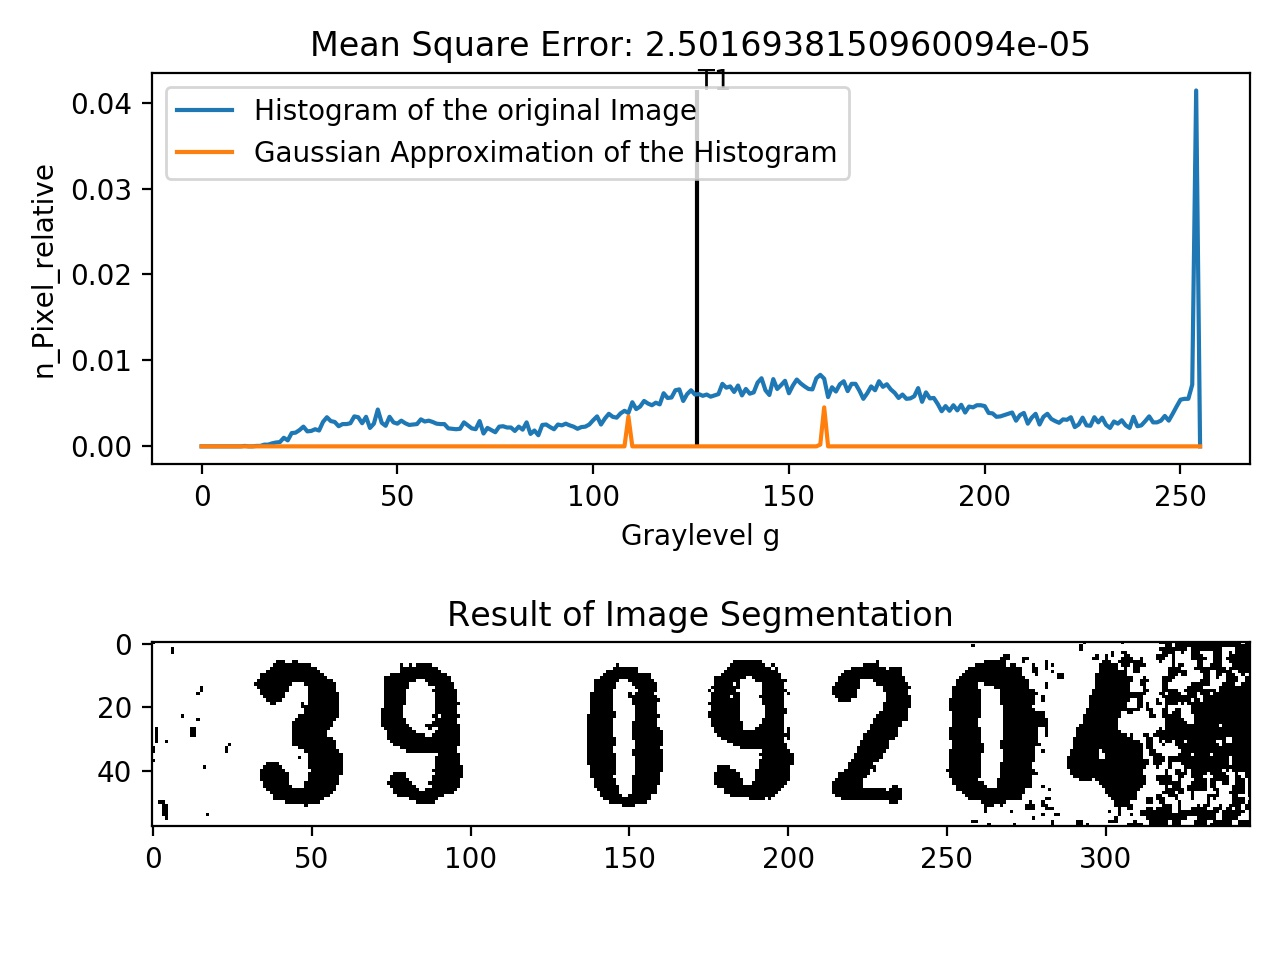
\includegraphics[width=0.52\linewidth]{vgl-4-1-1}}
				\subfloat[][K=2, G=20, Modell 2 ]{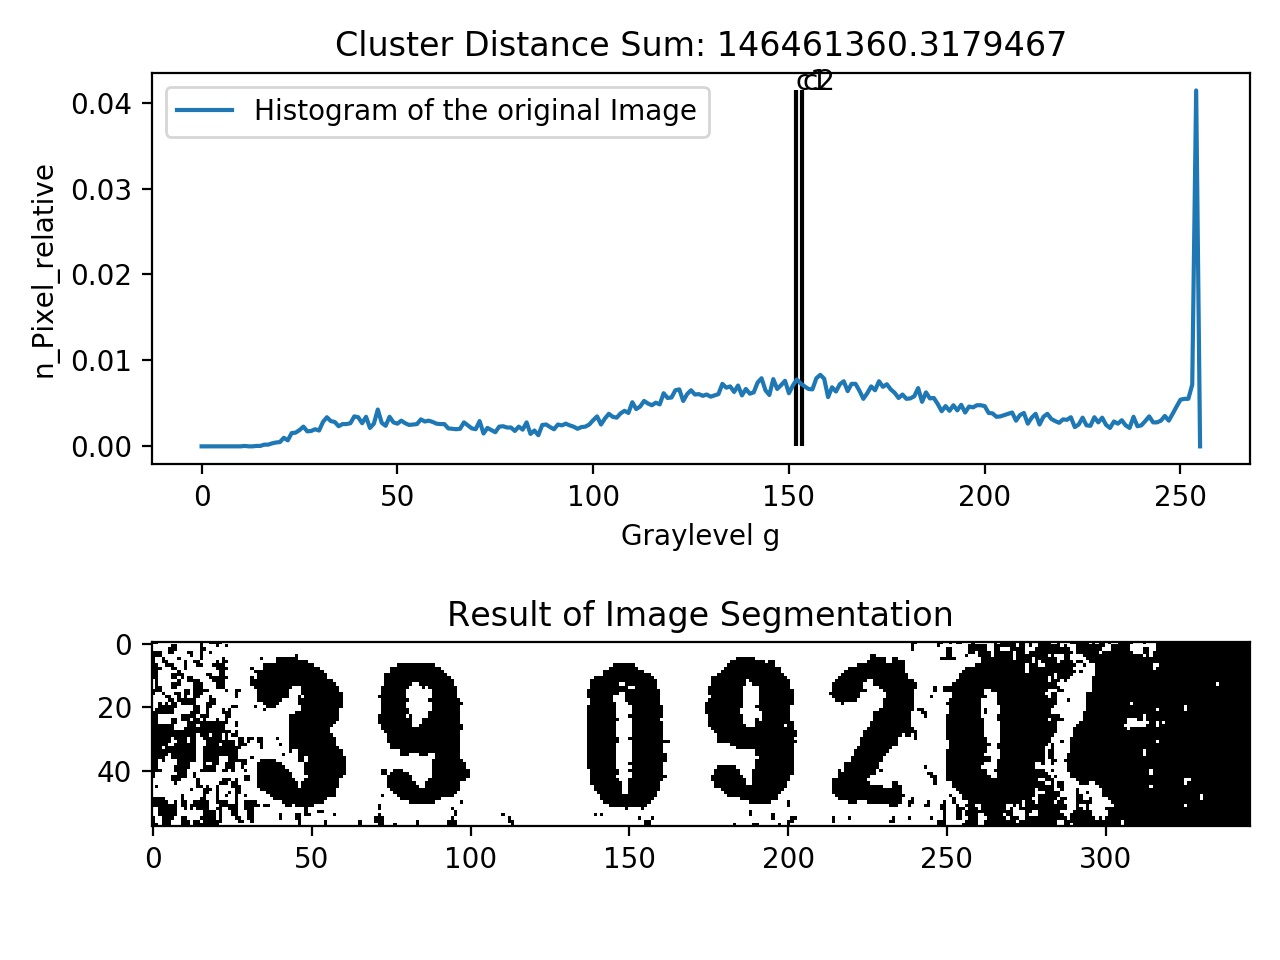
\includegraphics[width=0.52\linewidth]{vgl-4-1-2}}
				\caption{Beispiel-Plots mit gestempelten Bildern}
				\label{fig:vgl-4-1}
			\end{figure}
			Auf Abbildung \ref{fig:vgl-4-1} lässt sich erkennen, dass das Segmentierungsergebnis bei beiden Verfahren relativ verwertbar aussieht, wobei auf dem linken Bild der Text klarer zu erkennen ist, was ein korrektes Lesen mittels Tesseract erwarten lässt. \\
			Die Iterationszahlen sind jedoch sehr unterschiedlich, deswegen lässt sich das Ergebnis auf den ersten Blick nicht wirklich vergleichen. Wenn allerdings die Laufzeit mit in den Blick genommen wird, so wird der Unterschied rasant deutlich: für fünf Durchläufe auf Bildern mit gestempeltem Code benötigt Modell 1 lediglich 1,6 Sekunden, wohingegen Modell 2 das Zehnfache dieser Zeit beansprucht. Noch gravierender wiegt die Zeitdifferenz bei gelaserten Bildern, da diese einen größeren Dateiumfang besitzen. sind. Dafür benötigt Modell 2 beinahe vier Minuten, während sich für Modell 1 nichts ändert, da es nicht direkt auf dem Bild operiert, sondern auf dem Histogramm.\\
			Müsste vor diesem Hintergrund eine Entscheidung gefällt werden, würde die Wahl auf Modell 1 fallen, schlicht wegen der höheren Zeiteffizienz. Trotzdem ist es im Angesicht dieser niedrigen Erfolgsquoten unter anderem notwendig, die Parameter des \gls{de}-Algorithmus anzupassen, wozu wiederum ausgiebige Tests erforderlich sind, die allerdings den Rahmen dieser Arbeit sprengen würden.
		
		\subsection{Vergleich unterschiedlicher Bildgruppen}
		\label{sub:comp-diff-images}
			Insgesamt verläuft das Erkennen des Textes bei den gestempelten Bildern wesentlich erfolgreicher als bei den gelaserten Bildern. Dabei wurden 15\% der gestempelten Zeichencodes korrekt erkannt, während von den gelaserten Zeichensträngen nicht ein einziger vollständig erkannt werden konnte. 83\% von den erfolgreich gelesenen Bildern wurden vorher durch Verfahrensmodell 1 segmentiert, der Rest mit Modell 2.
			\begin{figure}[H]
				\centering
				\subfloat[][K=5, G=500, Modell 1 ]{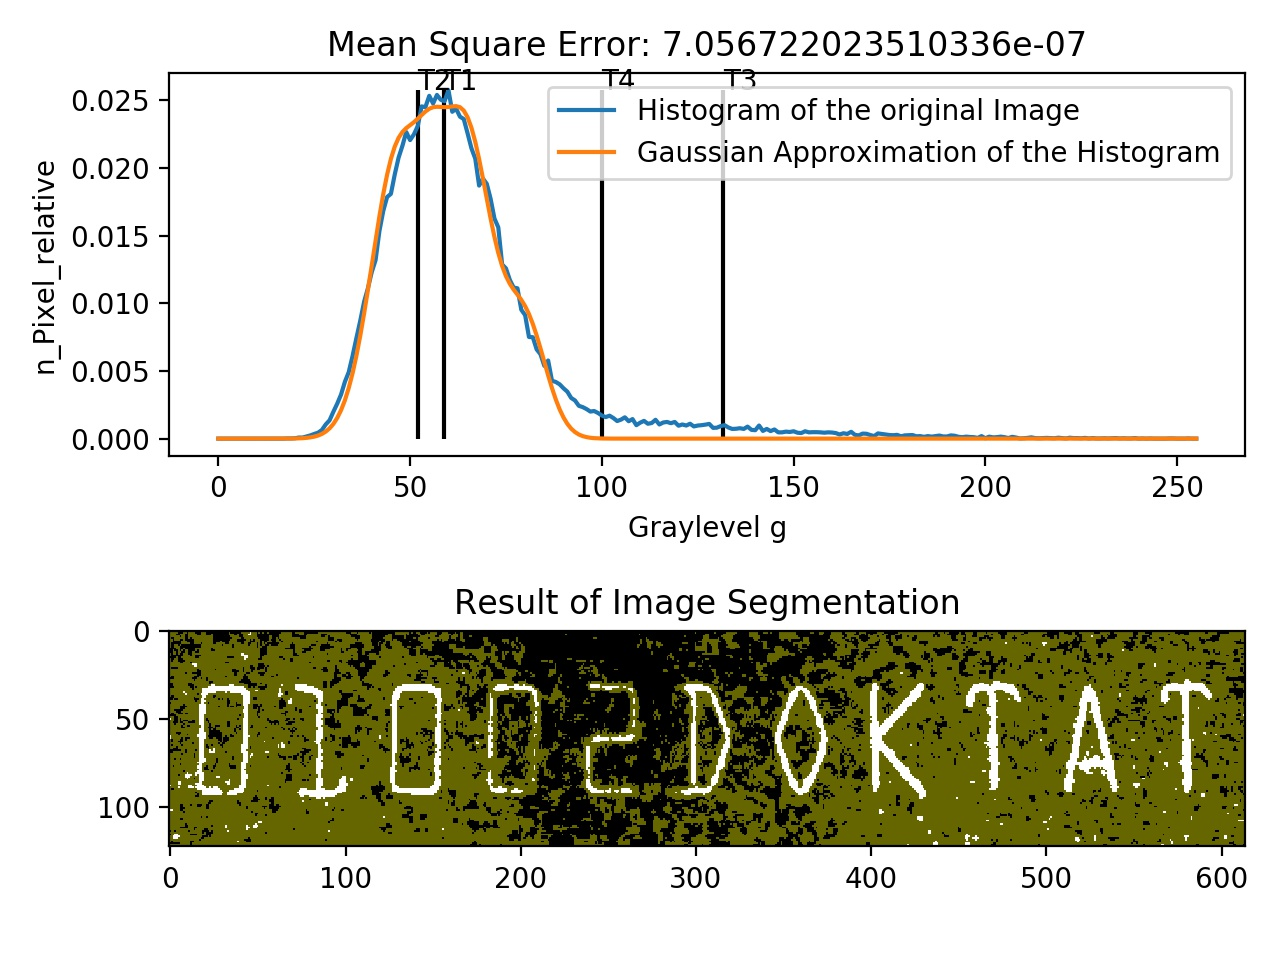
\includegraphics[width=0.52\linewidth]{vgl-4-2-1}}
				\subfloat[][K=5, G=500, Modell 1 ]{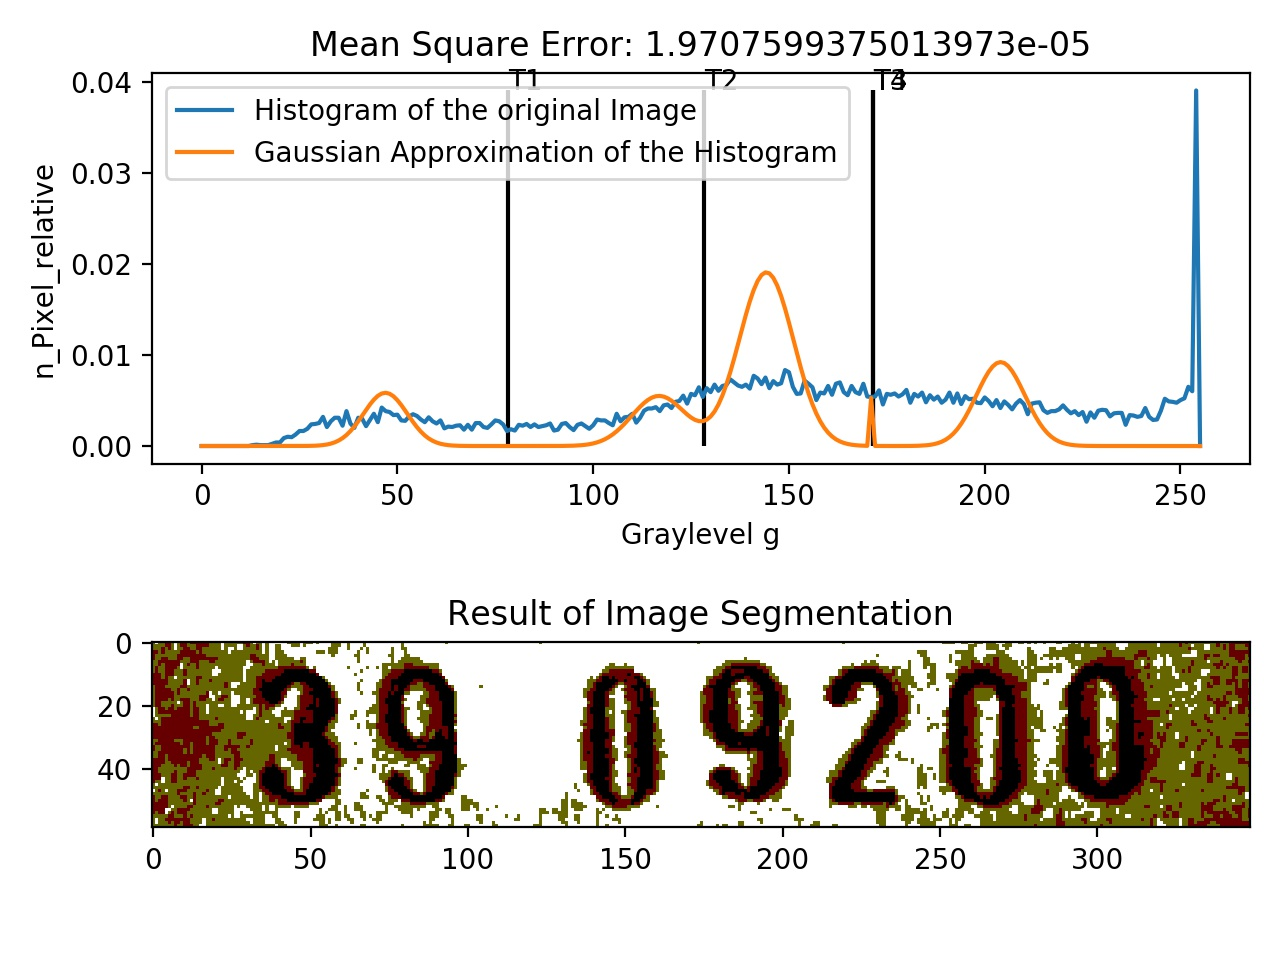
\includegraphics[width=0.52\linewidth]{vgl-4-2-2}}
				
				\subfloat[][K=5, G=10, Modell 2 ]{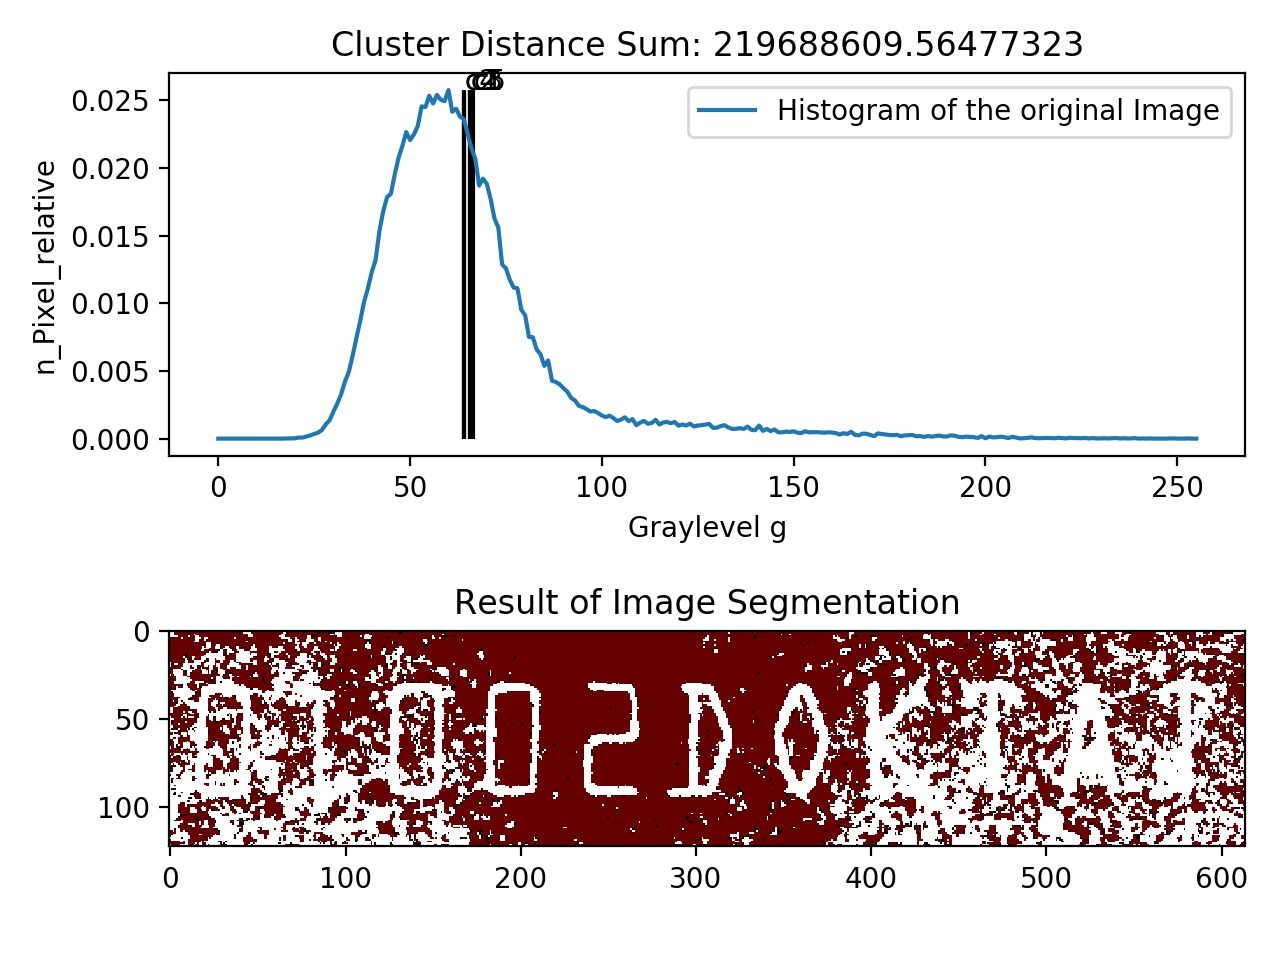
\includegraphics[width=0.52\linewidth]{vgl-4-2-3}}
				\subfloat[][K=5, G=10, Modell 2 ]{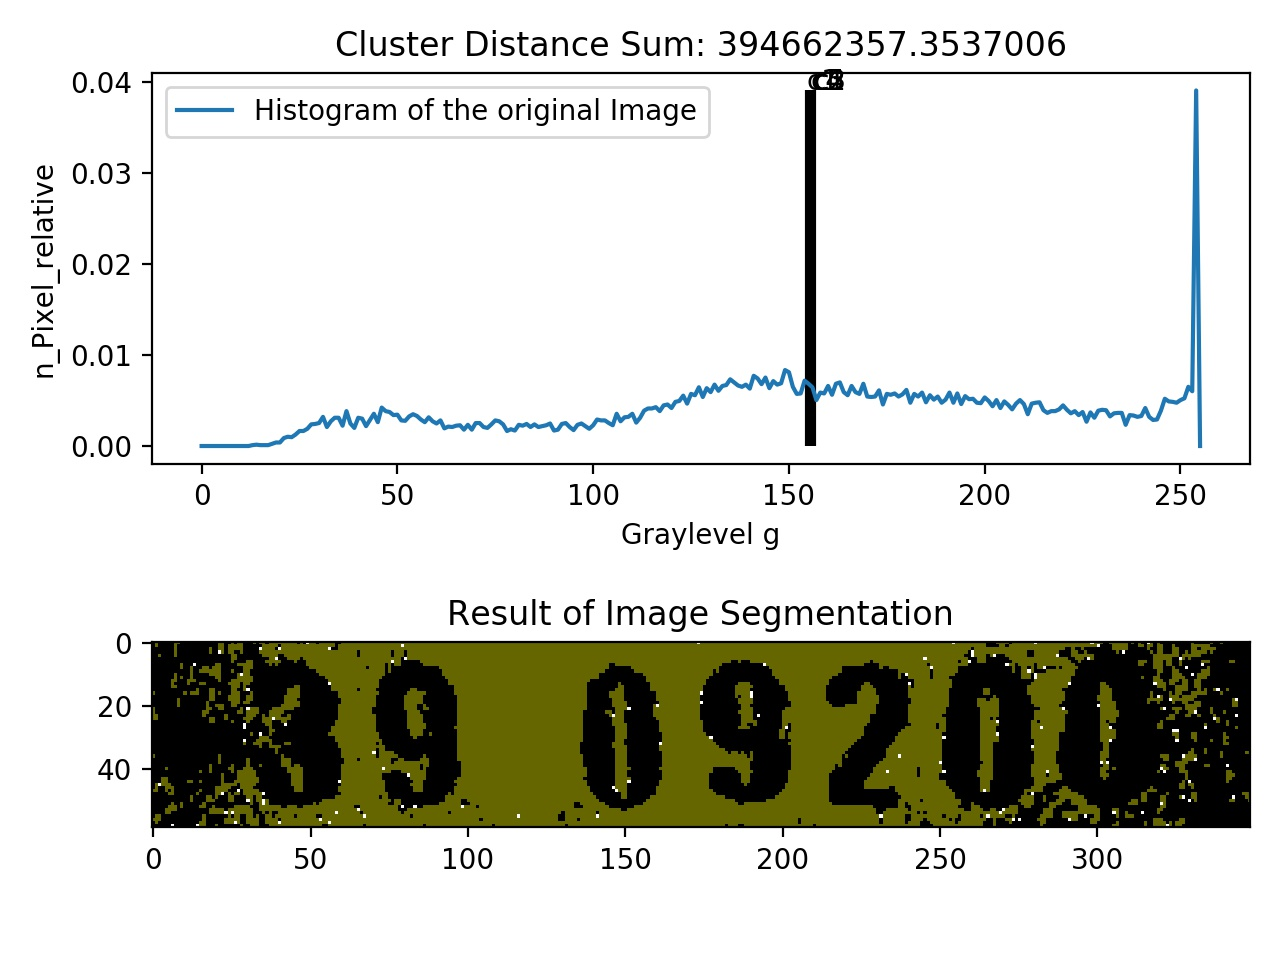
\includegraphics[width=0.52\linewidth]{vgl-4-2-4}}
				\caption{Gegenüberstellung Laser- und Stempel-Bilder}
				\label{fig:vgl-4-2}
			\end{figure}
			Die Sichtung von Abbildung \ref{fig:vgl-4-2} lässt zwei Vermutungen über das Auftreten des im oberen Absatz geschilderten Sachverhalts zu: \\
			Einerseits kommt zum Tragen, dass die lasergravierten Bilder ein höheres Rauschaufkommen aufweisen, wodurch sich nach der Segmentierung zahlreiche Artefakte bilden, die das Schriftbild für Tesseract verzerren. So kann es geschehen, dass Tesseract bei einer Eingabe wie auf folgender Abbildung \ref{fig:tesseract-fail} eine zusammenhanglose Zeichenkette zurückliefert:
			\begin{figure}[H]
				\centering
				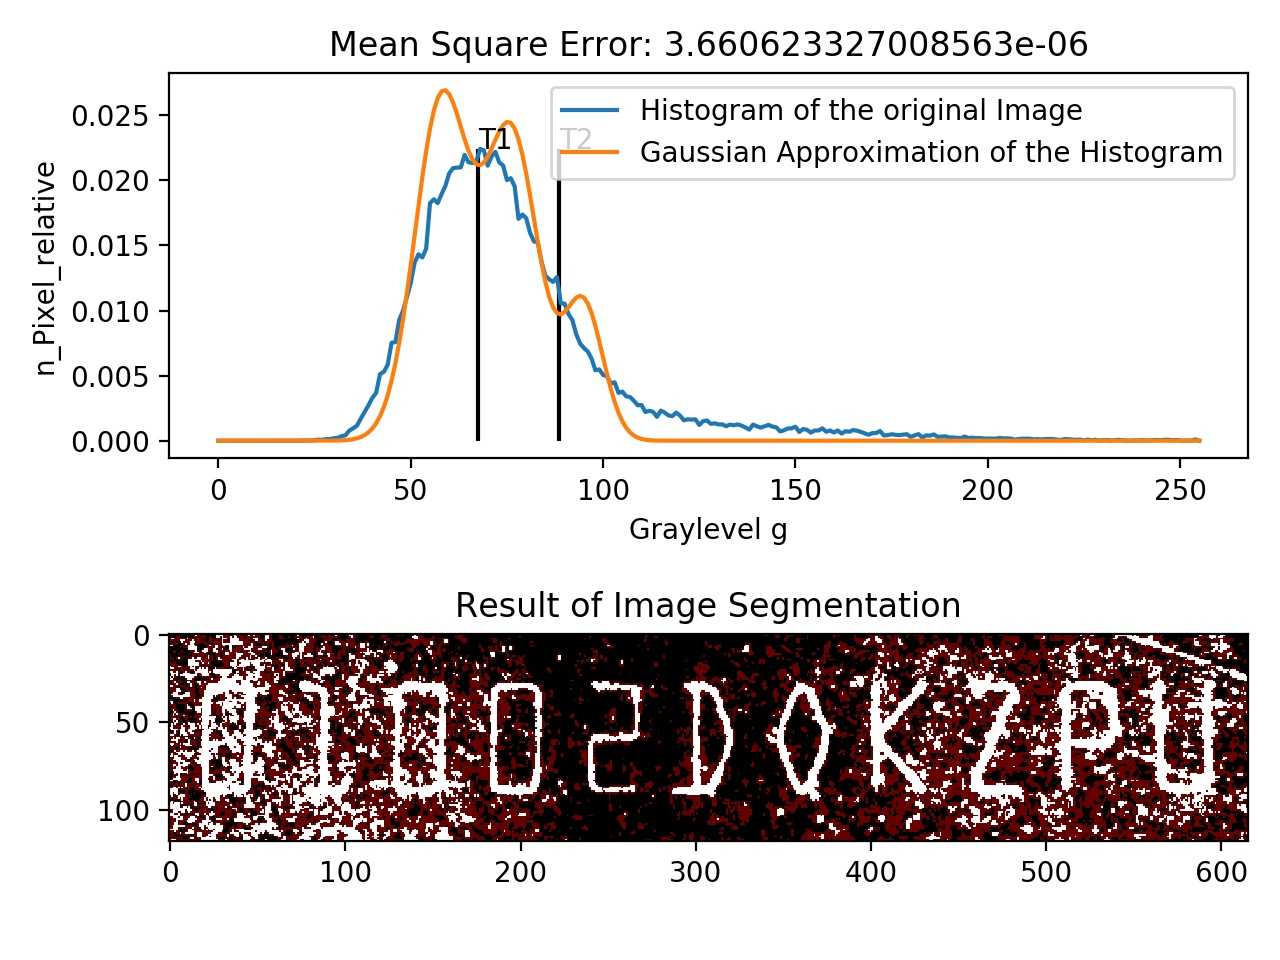
\includegraphics[width=0.7\linewidth]{tesseract-fail}
				\caption{Tesseract-Ausgabe: Hiaoohoniel (K=3, G=200, Modell 1)}
				\label{fig:tesseract-fail}
			\end{figure}
			Daneben gibt es einen anderen Spezialfall, der mitunter damit zusammenhängt, dass die Linienstärke der Zeichen bei den Stempel-Bildern merkbar höher ist als bei den Laser-Bildern. Dies sorgt beispielsweise dafür, dass Tesseract ein Zeichen, das eine Null darstellen soll, als ein \textbf{O} liest - so geschehen bei segmentiertem Bild in Abbildung \ref{fig:onechar-fail} als Input für Tesseract:
			\begin{figure}[H]
				\centering
				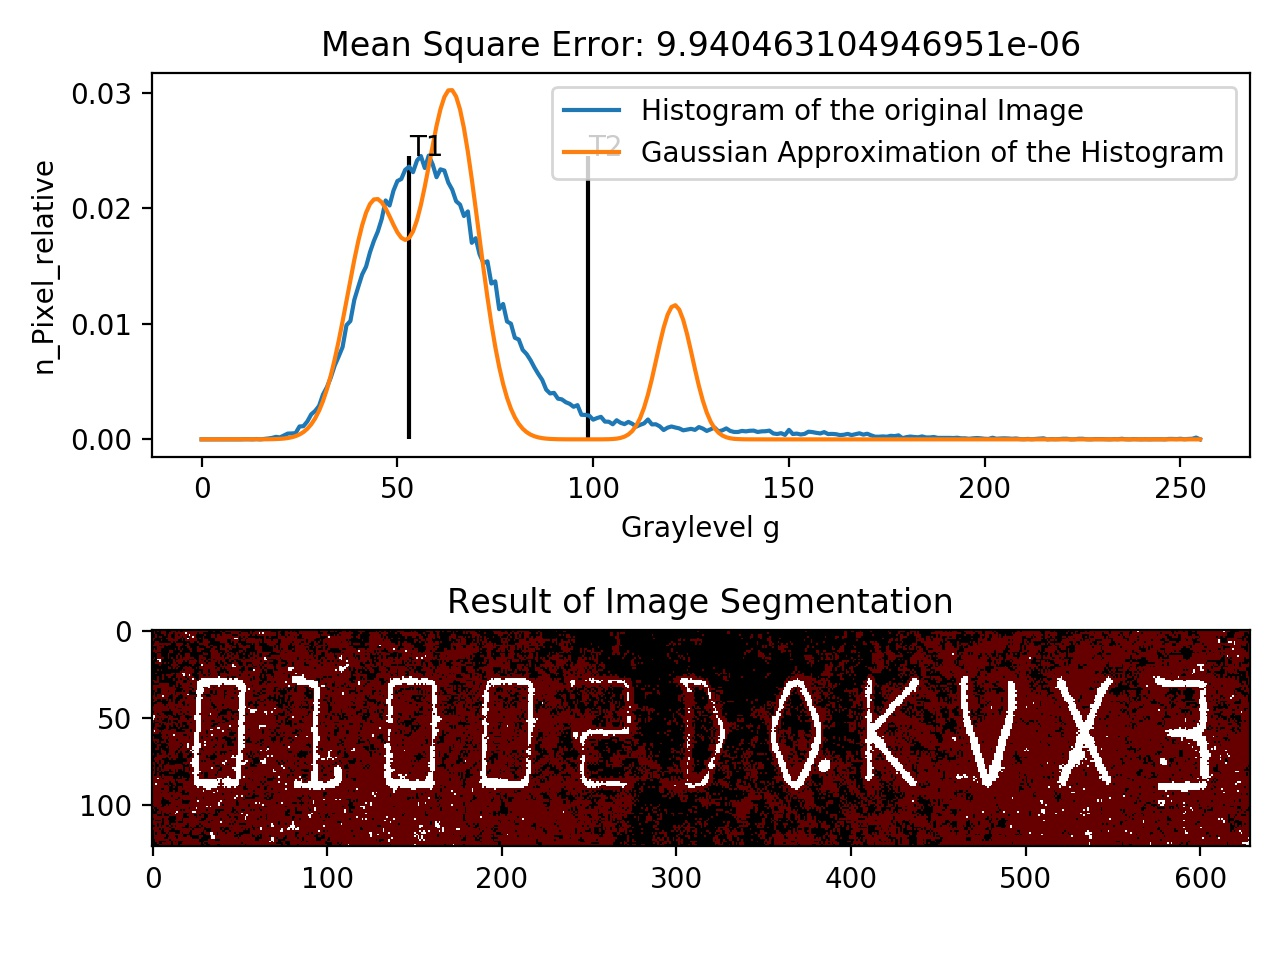
\includegraphics[width=0.7\linewidth]{onechar-fail}
				\caption{Tesseract-Ausgabe: 01002\textbf{00}KVX3 (K=3, G=100, Modell 1)}
				\label{fig:onechar-fail}
			\end{figure}
			An den Stellen, wo die beiden fettgedruckten Nullen positioniert sind, wurden ein \textbf{D} und ein \textbf{O} falsch gelesen.
		\subsection{Einfluss von Denoising auf das Ergebnis}
		\label{sub:influence-of-denoising}
			Entgegen der Erwartung, der Mittelwertfilter würde durch Rauschreduzierung das Erkennen des Textes erleichtern, wurden damit sogar weniger Codes korrekt gelesen. So waren nur 6\% der Versuche mit gefilterten Bildern erfolgreich, dahingegen wurden 9\% der Bilder, die nicht gefiltert worden sind, richtig gelesen. 
			\begin{figure}[H]
				\centering
				\subfloat[][K=4, G=500, Modell 1 ]{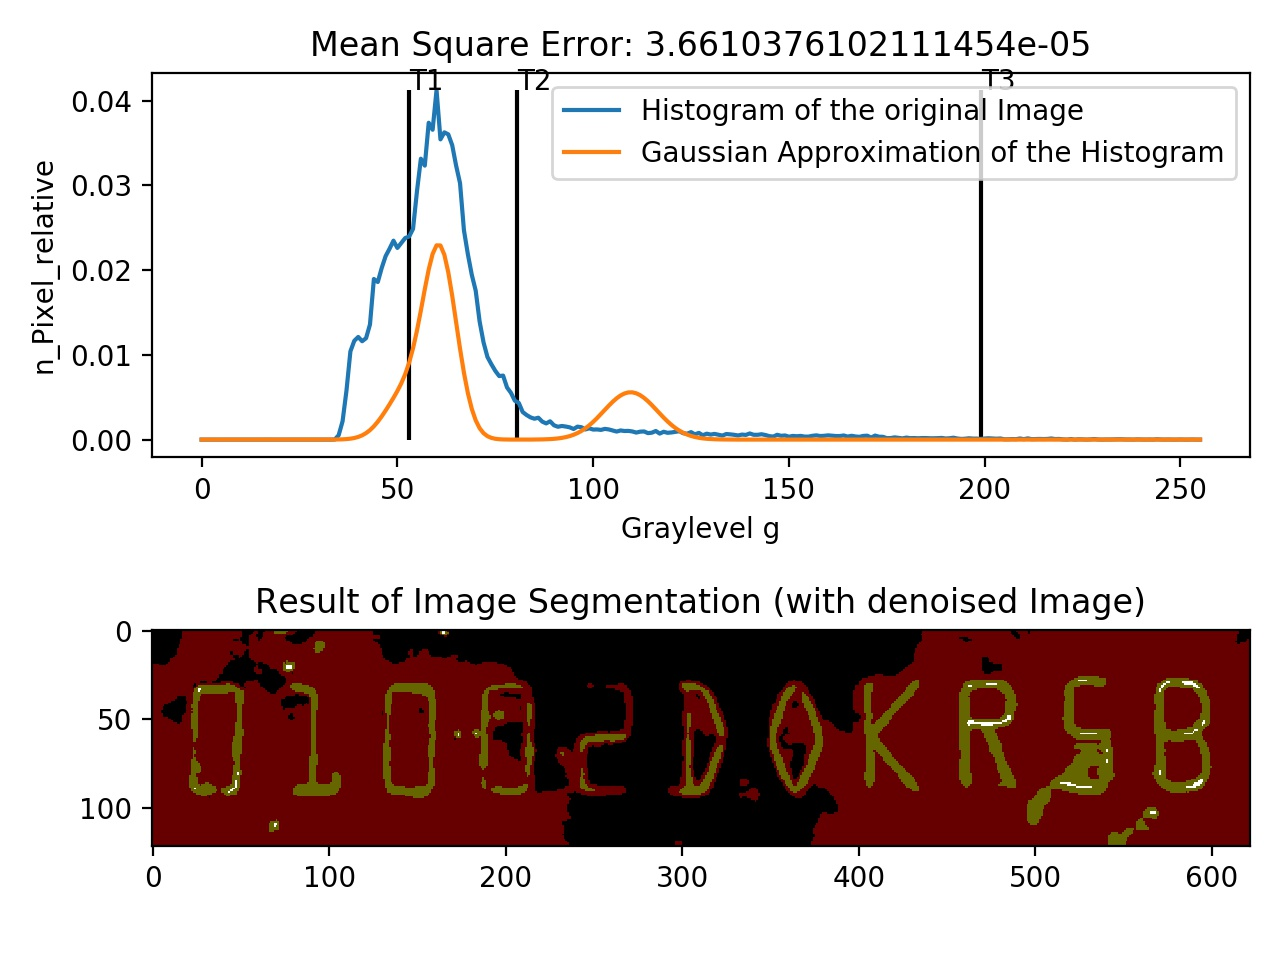
\includegraphics[width=0.52\linewidth]{vgl-4-3-1}}
				\subfloat[][K=4, G=500, Modell 1 ]{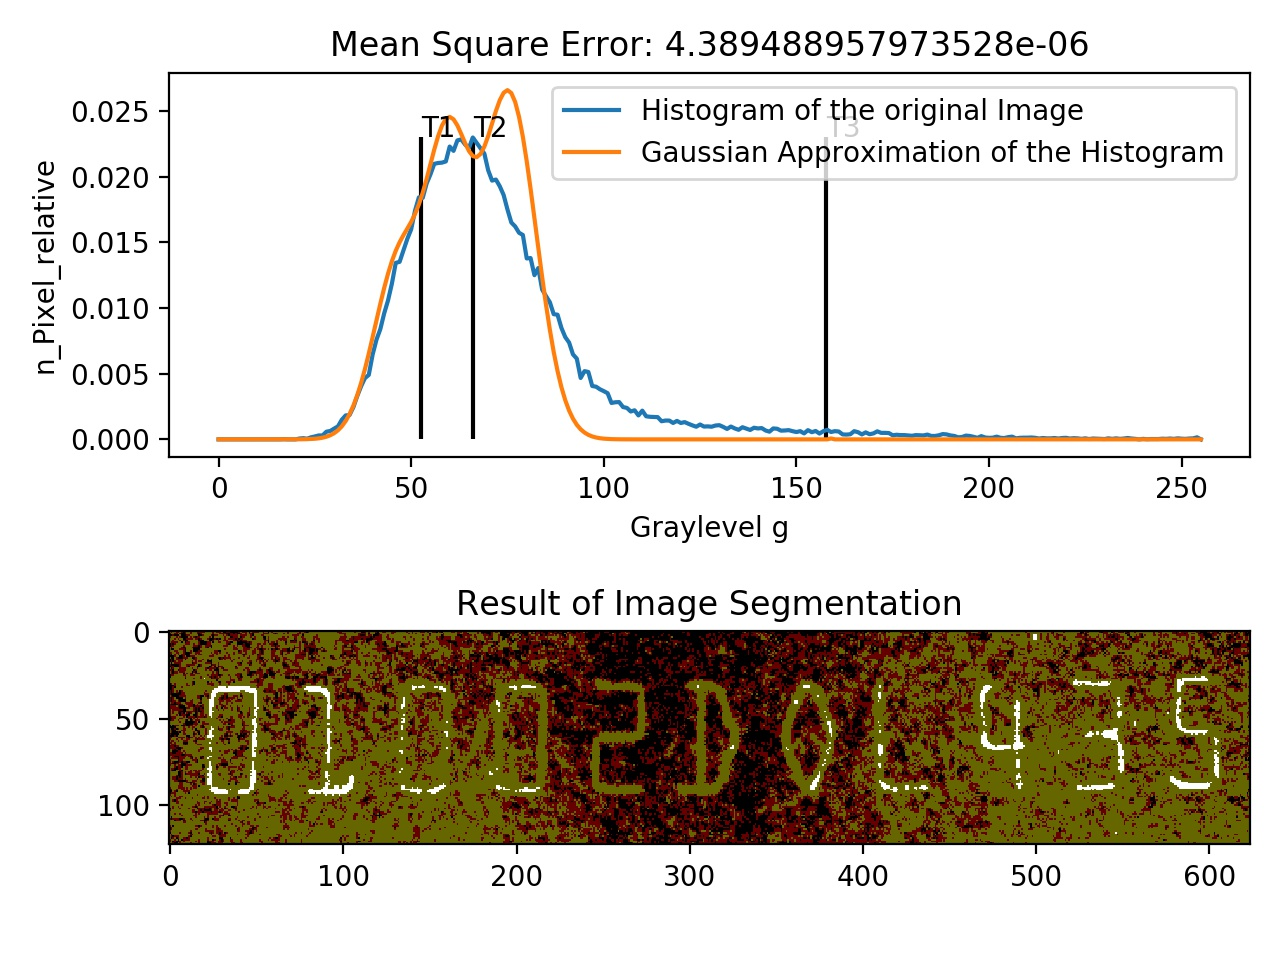
\includegraphics[width=0.52\linewidth]{vgl-4-3-2}}
				
				\subfloat[][K=4, G=500, Modell 1 ]{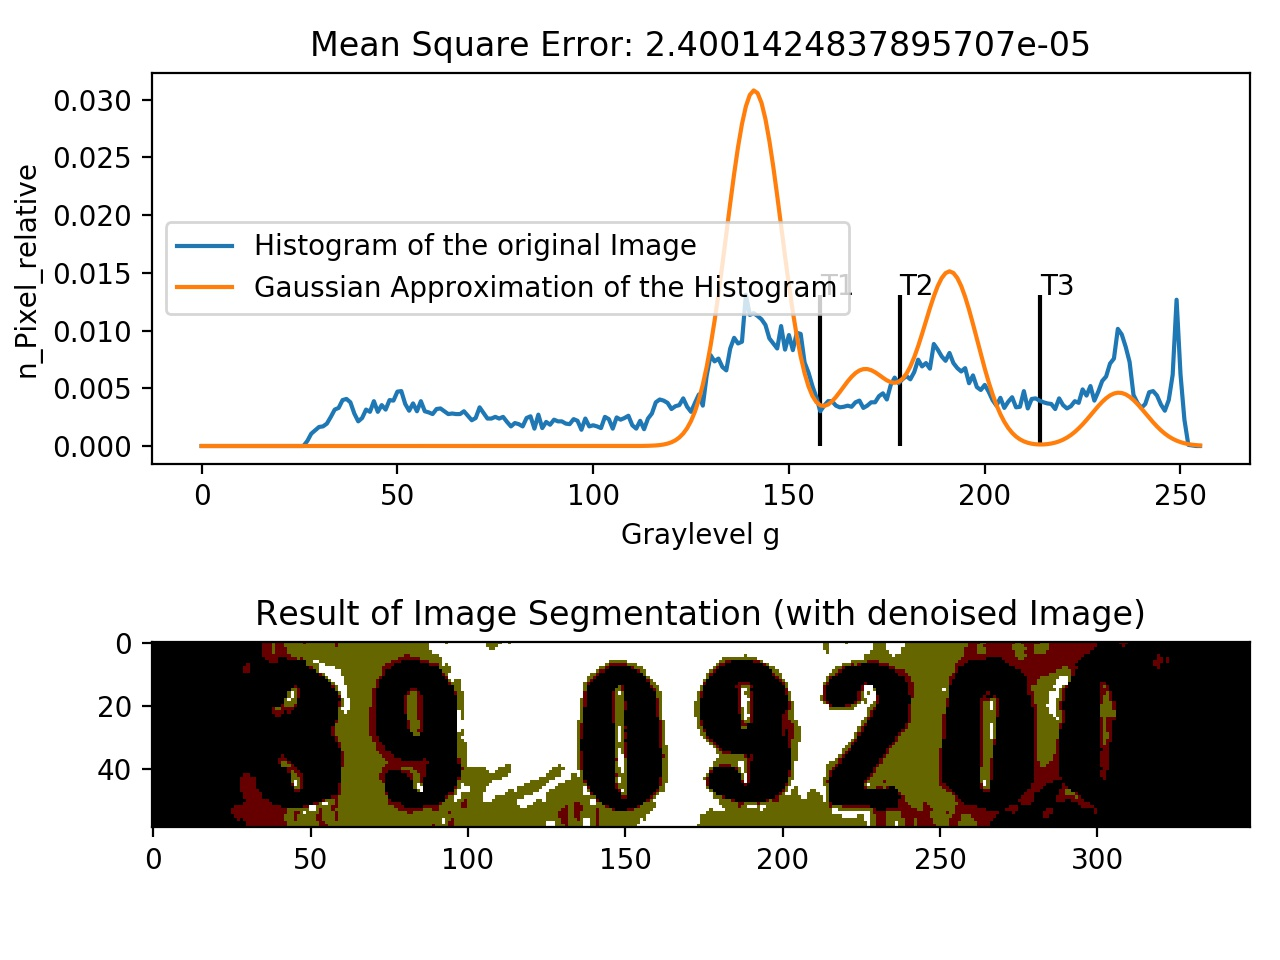
\includegraphics[width=0.52\linewidth]{vgl-4-3-3}}
				\subfloat[][K=4, G=500, Modell 1 ]{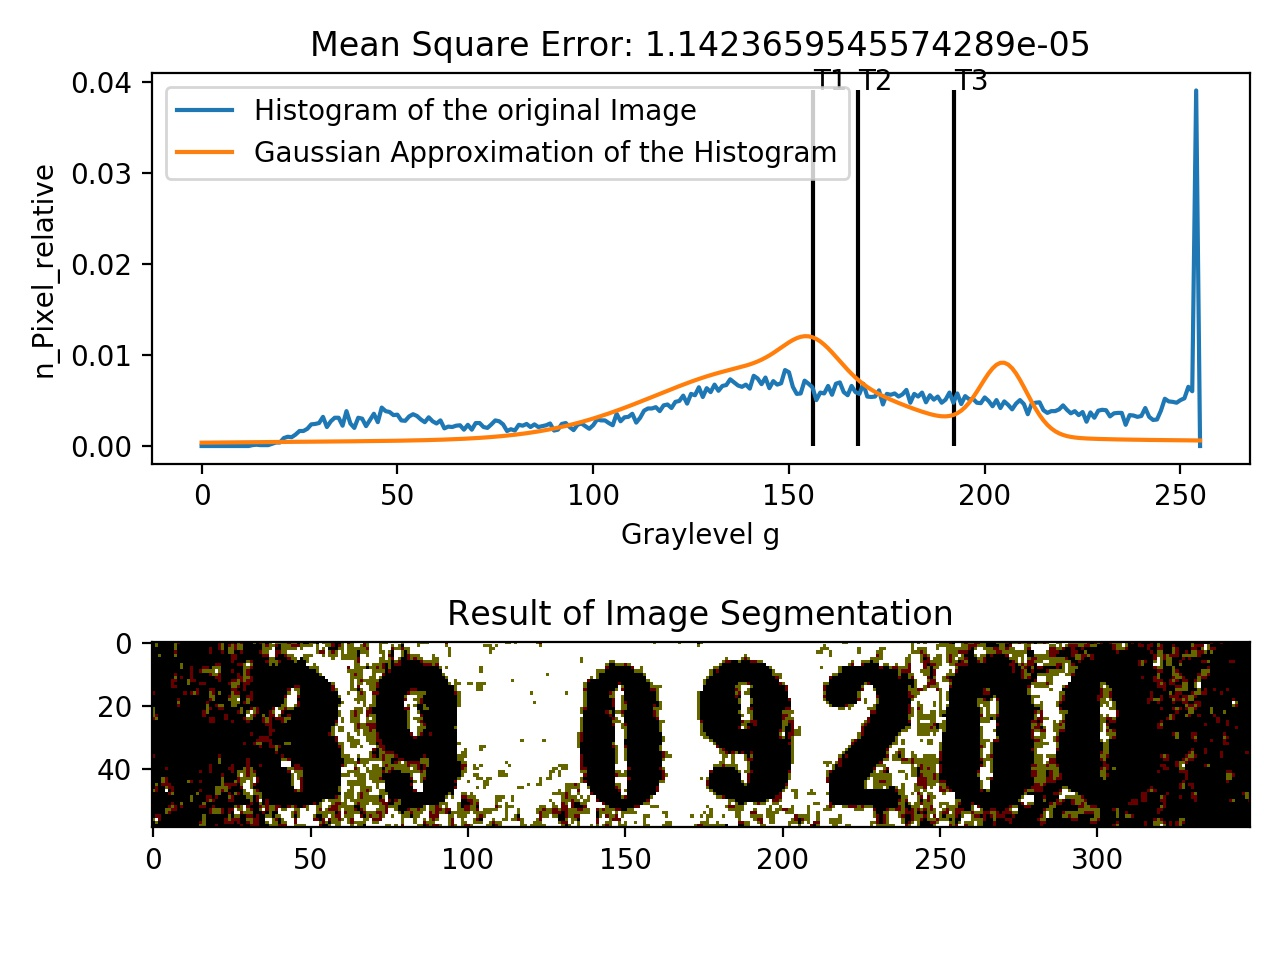
\includegraphics[width=0.52\linewidth]{vgl-4-3-4}}
				\caption{Gegenüberstellung gefilterte-nicht gefilterte Bilder (Modell 1) }
				\label{fig:denoise-compare1}
			\end{figure}
			Aus Abbildung \ref{fig:denoise-compare1} wird bei näherer Betrachtung der segmentierten Bilder ersichtlich, worin die Gefahr einer nicht behutsam angewendeten Mittelwertfilterung besteht. Zwar ist es richtig, dass der Mittelwertfilter benutzt werden kann, um eine Rauschreduktion zu erreichen. Jedoch geht dies auch mit einem Verlust an Kontrast einher. Im schlimmsten Fall kann dabei sogar ein Teil der Information verloren gehen. 
		
		\subsection{Einfluss der Klassenanzahl auf das Ergebnis}
		\label{sub:influence-of-classes}
			An dieser Stelle steht die Frage im Raum, ob es sinnvoll ist, eine Segmentierung in mehr als zwei Klassen durchzuführen. Im Allgemeinen ist dies anwendungsabhängig. Spezifiziert auf diese Arbeit würde die Antwort auf die vorherige Frage tendenziell negativ ausfallen. Denn im Vergleich konnten die Segmentierungsversuche in zwei Klassen bei einer Erfolgsquote von 14\% die größten Erfolge erzielen. Im Gegensatz dazu haben die Versuche mit vier Klassen mit 1\% die niedrigste Erfolgsrate. Diejenigen Versuche mit drei und jene mit fünf Klassen bilden mit 8\% und 5\% die Mitte. 
			\begin{figure}[H]
				\centering
				\subfloat[][K=2, G=1000, Modell 1 ]{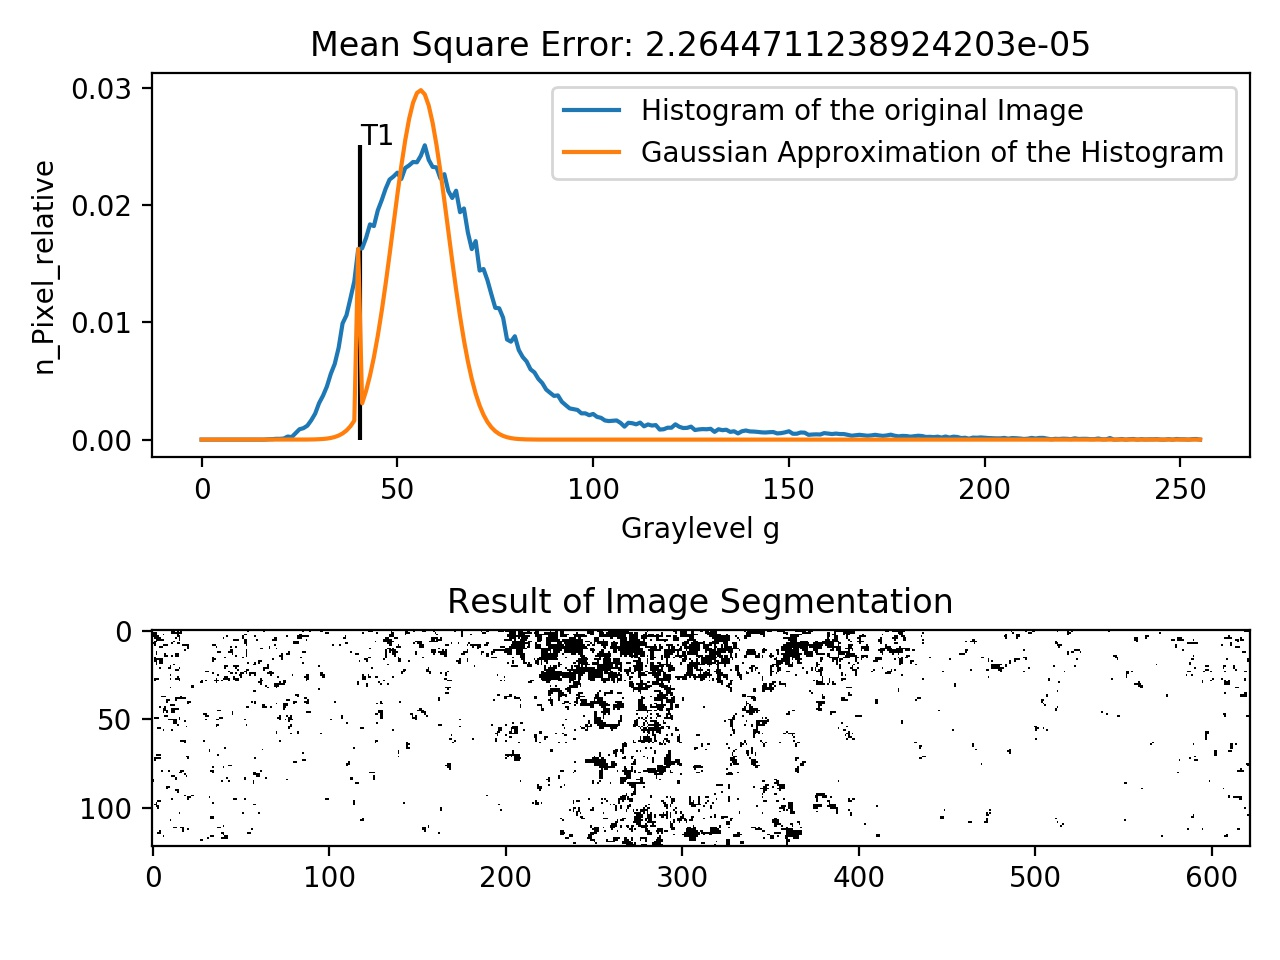
\includegraphics[width=0.52\linewidth]{vgl-4-4-1}}
				\subfloat[][K=3, G=1000, Modell 1 ]{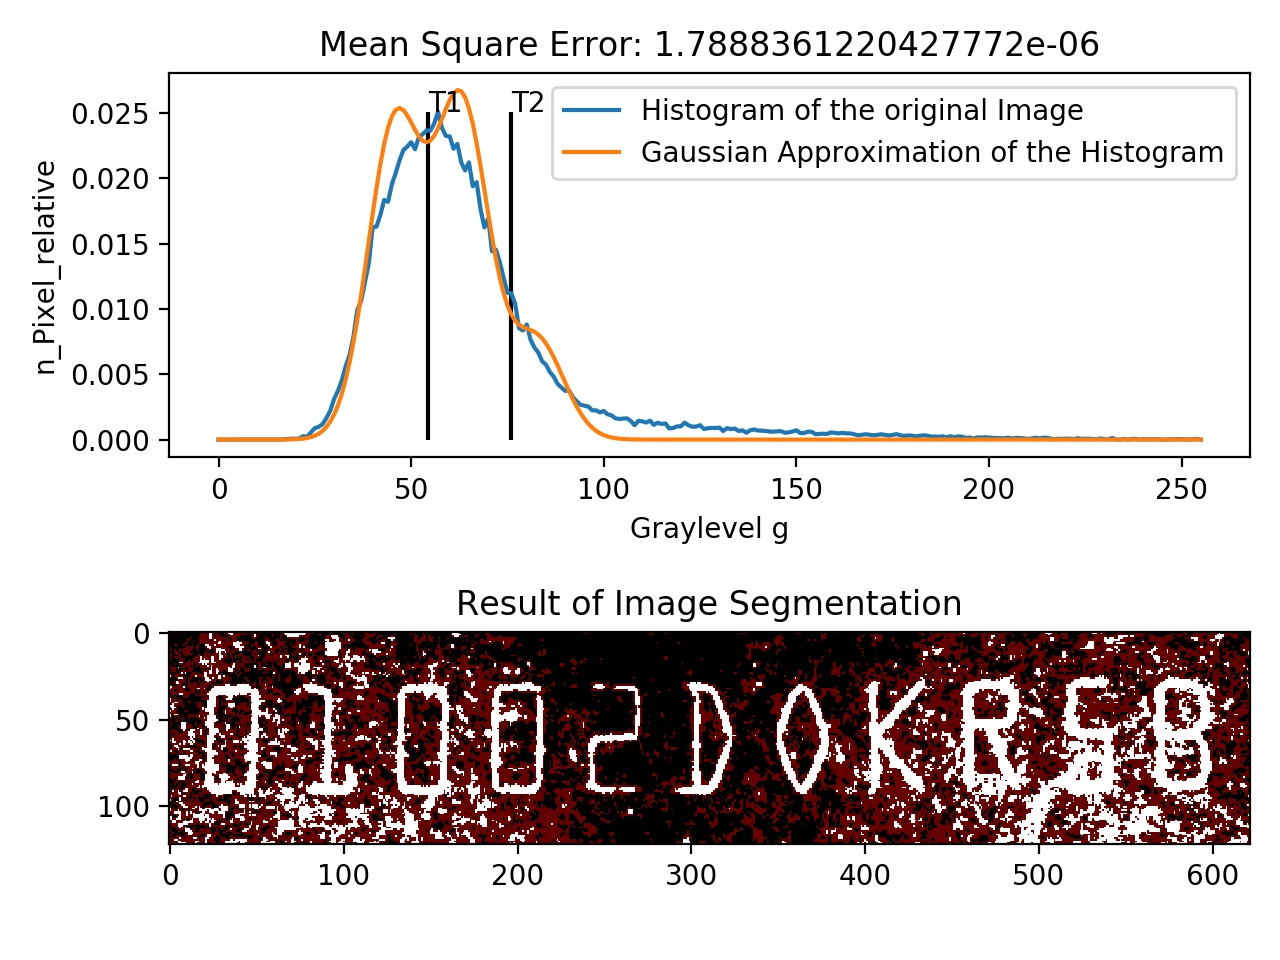
\includegraphics[width=0.52\linewidth]{vgl-4-4-2}}
				
				\subfloat[][K=4, G=1000, Modell 1 ]{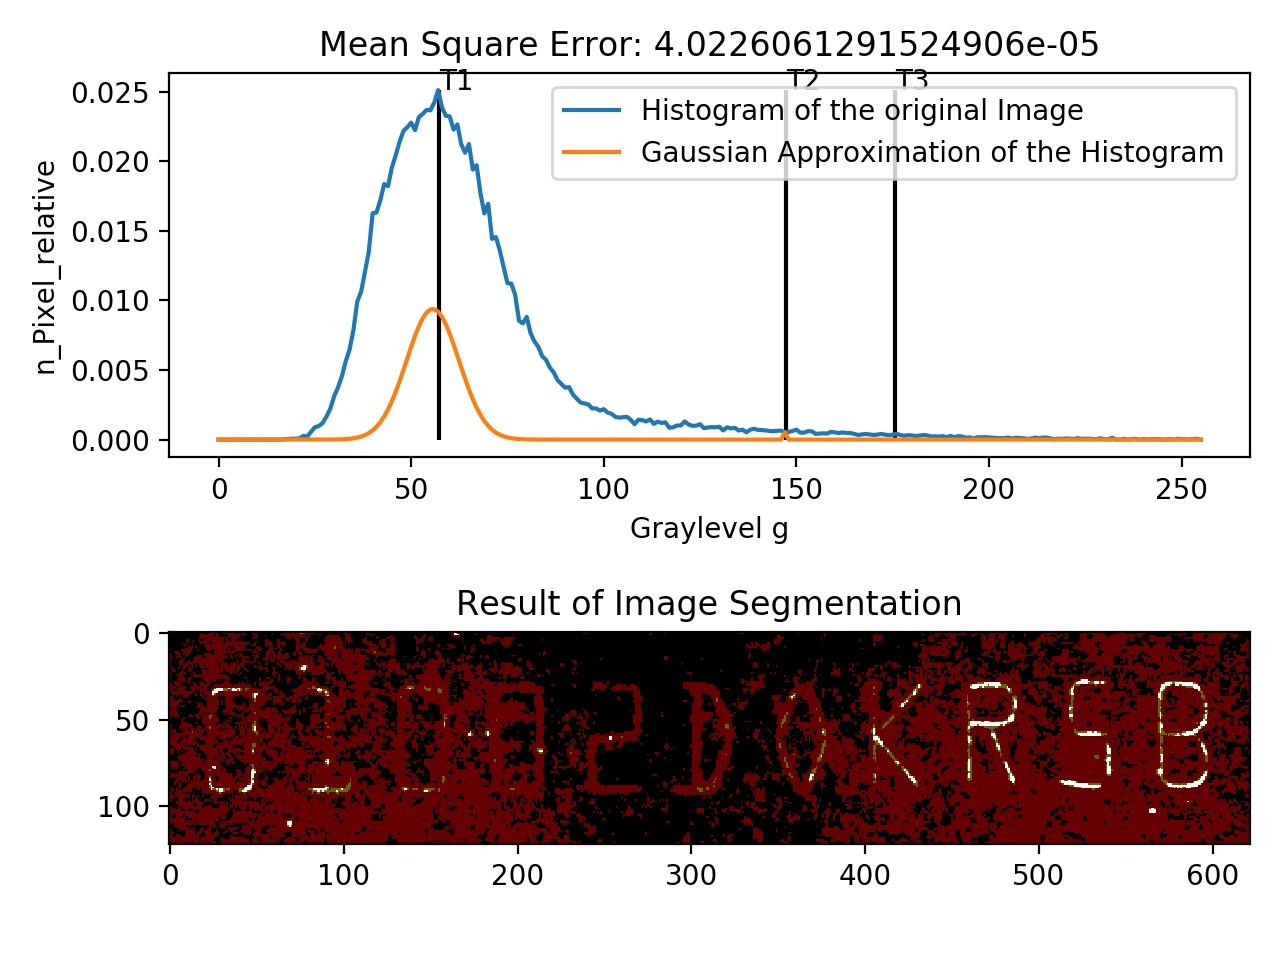
\includegraphics[width=0.52\linewidth]{vgl-4-4-3}}
				\subfloat[][K=5, G=1000, Modell 1 ]{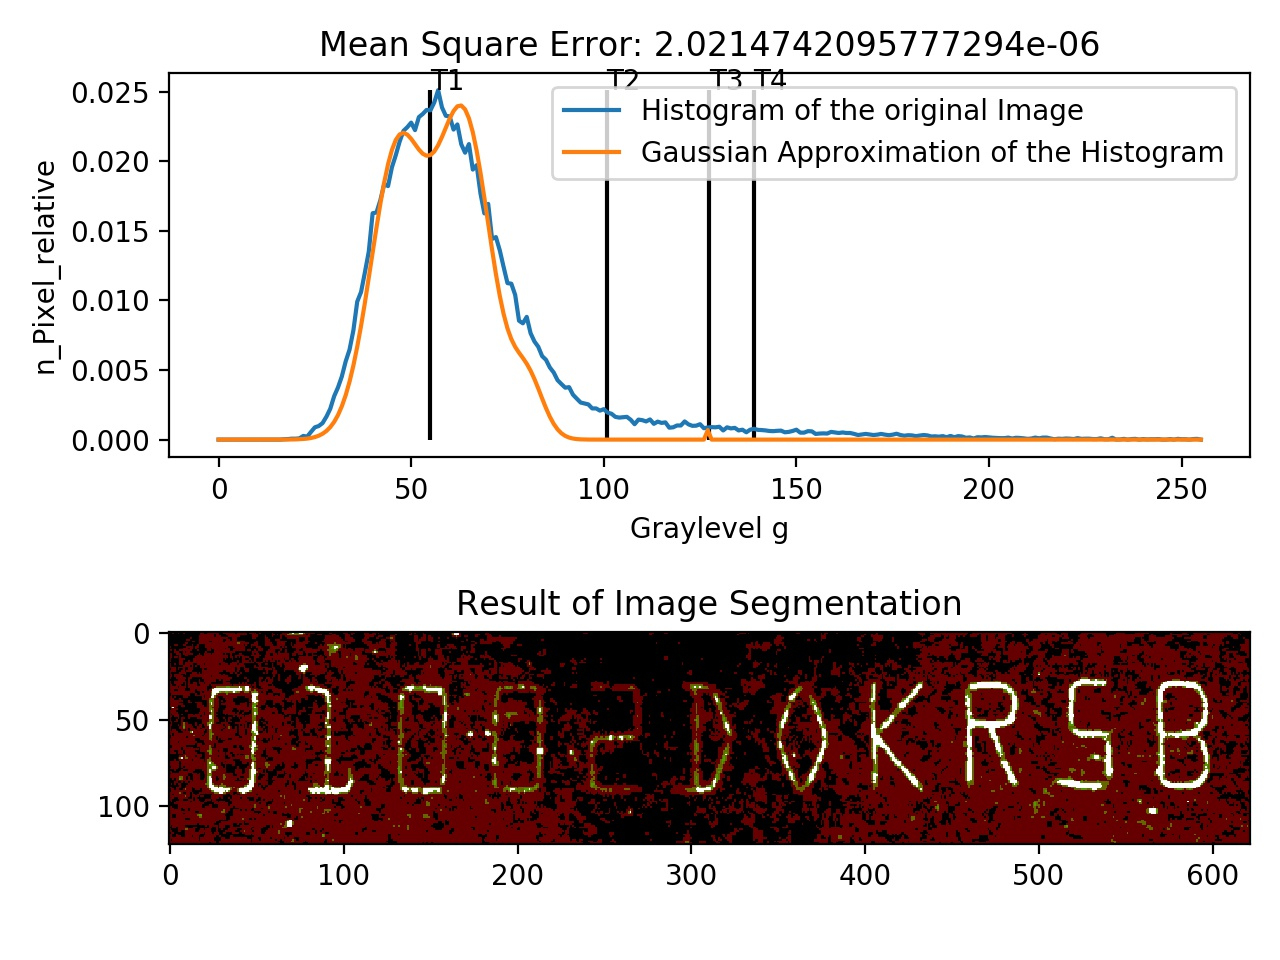
\includegraphics[width=0.52\linewidth]{vgl-4-4-4}}
				\caption{Gegenüberstellung Klassen (Modell 1) }
				\label{fig:classes-compare1}
			\end{figure}
			Bei eingehender Inspektion der Linienplots in Abbildung \ref{fig:classes-compare2} lässt sich festhalten, dass Segmentierungsmodell 1 insofern von einer höheren Klassenanzahl, dass die Approximation des Histogramms über eine Summe Gaußscher Normalverteilungsfunktionen dementsprechend neue Summenglieder erhält und somit das Histogramm genauer approximieren.
			\begin{figure}[H]
				\centering
				\subfloat[][K=2, G=10, Modell 2 ]{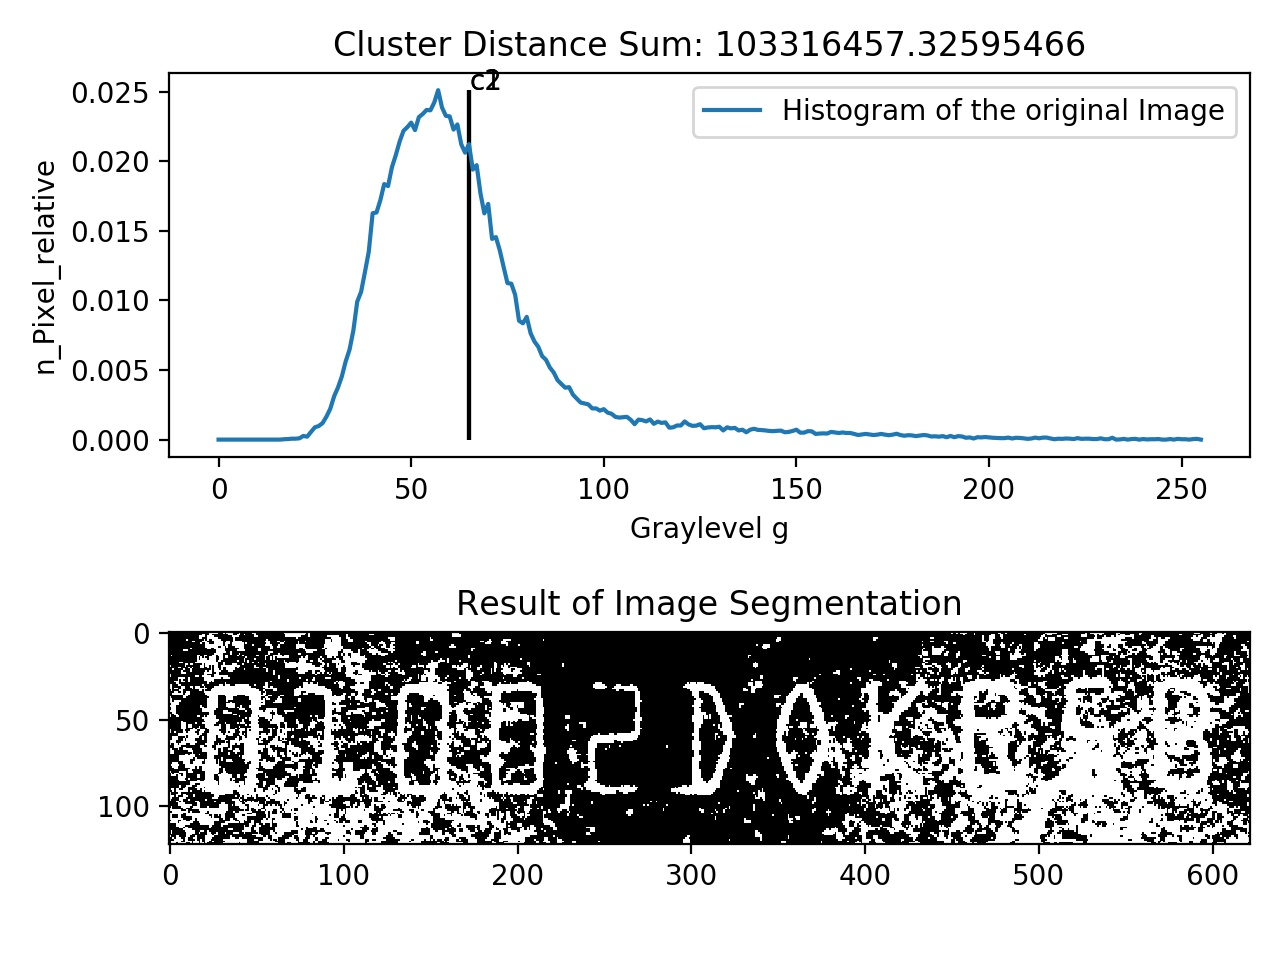
\includegraphics[width=0.52\linewidth]{vgl-4-4-5}}
				\subfloat[][K=3, G=10, Modell 2 ]{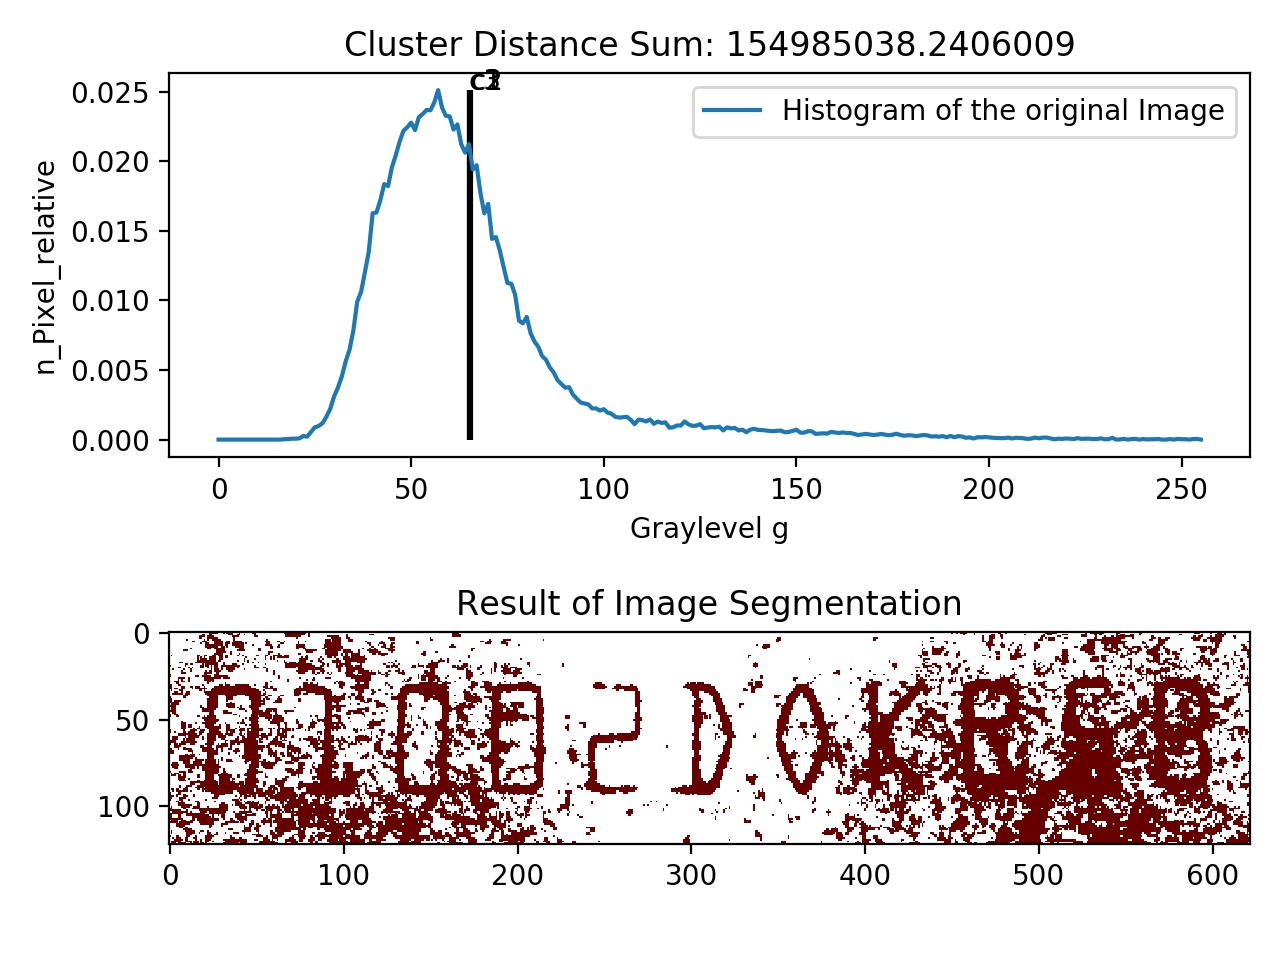
\includegraphics[width=0.52\linewidth]{vgl-4-4-6}}
				
				\subfloat[][K=4, G=10, Modell 2 ]{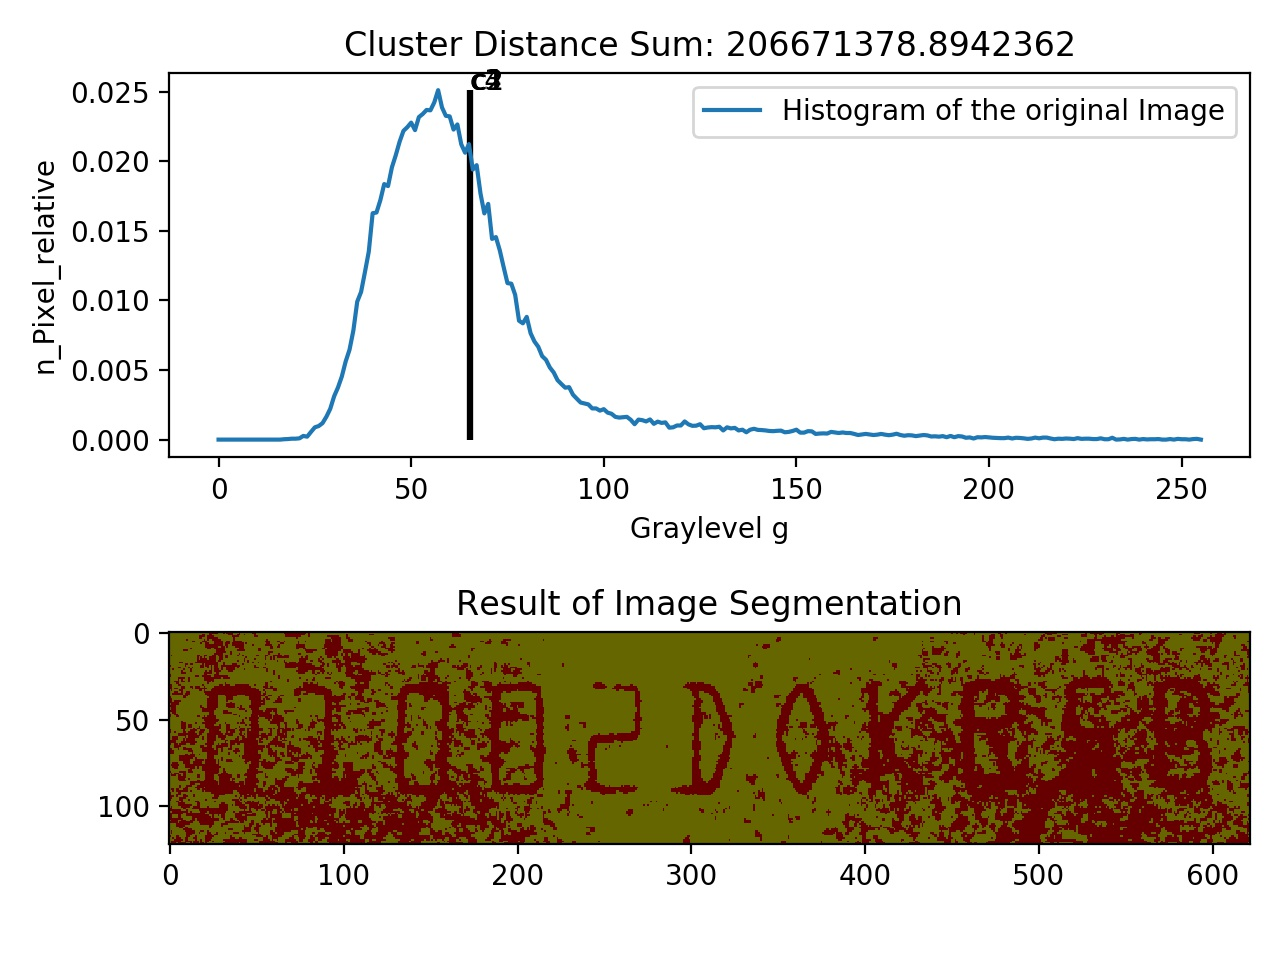
\includegraphics[width=0.52\linewidth]{vgl-4-4-7}}
				\subfloat[][K=5, G=10, Modell 2 ]{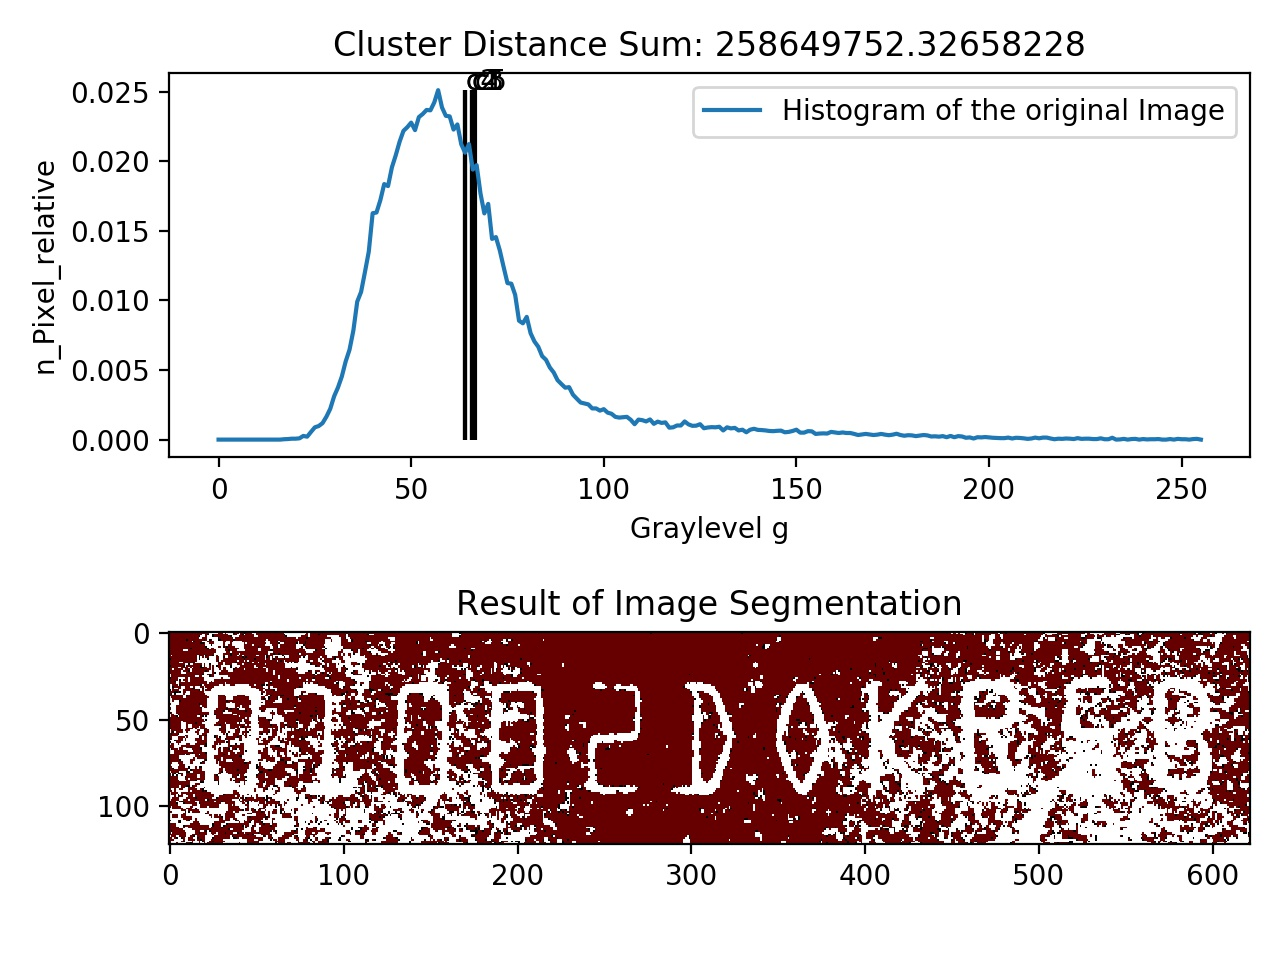
\includegraphics[width=0.52\linewidth]{vgl-4-4-8}}
				\caption{Gegenüberstellung Klassen (Modell 2) }
				\label{fig:classes-compare2}
			\end{figure}
			Auf Abbildung \ref{fig:classes-compare2} sieht man wiederum einen Vergleich der Ergebnisse bei unterschiedlichen Klassen, diesmal nur für Segmentierungsmodell 2. Ein nennenswerter Effekt ist dort nicht erkennbar.
			
		\subsection{Verhalten bei steigender Iterationszahl}
		\label{sub:behav-rising-it}
			